\documentclass[conference]{IEEEtran}
\IEEEoverridecommandlockouts

\usepackage{cite}
\usepackage{amsmath,amssymb}
\usepackage{graphicx}
\usepackage{booktabs}
\usepackage{multirow}
\usepackage{array}
\newcolumntype{L}[1]{>{\raggedright\arraybackslash}p{#1}}
\usepackage{xcolor}
\usepackage{url}
\usepackage{tikz}
\usetikzlibrary{arrows.meta,positioning,fit,calc}
\usepackage{pgfplots}
\pgfplotsset{compat=1.17}

\definecolor{shieldteal}{HTML}{0B8FA6}
\definecolor{shieldnavy}{HTML}{1D2B47}
\definecolor{shieldgrey}{HTML}{B7C2D3}
\newcommand{\code}[1]{\texttt{\small #1}}

\begin{document}

\title{GraphQL-Shield: Schema-Aware Dual-Layer Enforcement Against GraphQL BOLA with Self-Supervised Blind-Spot Detection}

\author{
\IEEEauthorblockN{[Author 1]}
\IEEEauthorblockA{[Department, Institution]\\ {[City, Country]}\\ {[email]}}
\and
\IEEEauthorblockN{[Author 2]}
\IEEEauthorblockA{[Department, Institution]\\ {[City, Country]}\\ {[email]}}
\and
\IEEEauthorblockN{[Author 3]}
\IEEEauthorblockA{[Department, Institution]\\ {[City, Country]}\\ {[email]}}
}

\maketitle

\begin{abstract}
Broken Object Level Authorization (BOLA) is the top risk in the OWASP API Security Top~10, and GraphQL makes it harder to stop: a single request can reach an object by its identifier, through nested lookups, inside fragments, variables and batches, or through relationship fields that never name the object at all. We present GraphQL-Shield, a gateway that enforces object ownership at two independent points: a schema-aware pre-execution layer that checks every object identifier it can resolve before any resolver runs, and an execution-time layer that checks every object the resolvers return and every mutation target the engine coerces. The second layer also measures the first: each object it evaluates that the first layer never saw is recorded, and these cross-layer disagreements become training labels, with no manual labelling, for a model that predicts the first layer's blind spots from query structure alone. On 4,000 generated requests the model exposed a previously unknown bypass of the first layer (variable default values) that a hand-written rule missed entirely; fixing it cut attacks stoppable only by the second layer by 66\%. Both layers are configured from the schema and a small ownership map and protect a second, unrelated application without code changes. Compared with graphql-shield on the same schema and scenarios, GraphQL-Shield leaks no object, blocks no legitimate request where graphql-shield loses an owner's own data to GraphQL null propagation, and needs 3 configuration entries instead of 12. After connection pooling, in-process overhead is 60--81\% over an unprotected endpoint.
\end{abstract}

\begin{IEEEkeywords}
GraphQL, API security, broken object level authorization, access control, defense in depth, machine learning, self-supervised learning
\end{IEEEkeywords}

% ===================================================================
\section{Introduction}

An API has a BOLA flaw when it returns or changes an object without checking that the caller may access it. OWASP ranks it first among API risks (API1:2023)~\cite{owasp2023}, and it is hard to detect because a BOLA request is ordinary authenticated traffic: the only difference is whose object it names.

GraphQL widens this attack surface. A REST endpoint usually takes one object identifier in its path; a GraphQL request can name many objects at any depth and can reach objects without naming them. A caller who owns a folder can list its \code{children}, including a document owned by someone else, and no identifier for that document ever appears in the query. The same identifier can also arrive as a literal, a variable, a variable's default value, inside a named or inline fragment, under an alias, or in one operation of a batch.

Two families of defence exist, and each misses something. Checks that analyse the query before execution see only the identifiers written in it, so relationship traversal is invisible to them. Checks written into each resolver see every object but must be written and maintained field by field. We show both effects experimentally: a pre-execution layer alone leaks relationship traversal (Section~\ref{sec:ablation}), and per-field rules either execute an unprotected write or block legitimate requests when one rule is missing (Section~\ref{sec:comparison}).

GraphQL-Shield combines both and uses each to audit the other. Our contributions are:
\begin{enumerate}
\item \textbf{Dual-layer enforcement with cross-layer evidence.} A schema-aware pre-execution layer and an execution-time layer enforce ownership independently; the second records every object the first never evaluated, so the gateway measures its own pre-execution coverage.
\item \textbf{Self-supervised blind-spot prediction.} These records label requests automatically. A gradient-boosted model trained on them predicts the first layer's blind spots before execution and explains them per feature. Its discovery run found a previously unknown bypass; the fix cut attacks reaching only the second layer by 66\%.
\item \textbf{Schema-driven, portable configuration.} Both layers read owned types, relationship fields and mutation targets from the schema and a small ownership map, run as graphql-core middleware, and handle Relay global identifiers, including type-confused ones. The same layers protect a second, unrelated application.
\item \textbf{Evaluation.} Layer ablation, a comparison with graphql-shield on the same schema and scenarios including configuration mistakes, latency with confidence intervals, and multi-seed evaluation of the predictor.
\end{enumerate}

% ===================================================================
\section{Background}

\textbf{GraphQL execution.} A GraphQL server parses a request, validates it against a typed schema, and calls a resolver for each selected field, top down. Arguments are coerced first: variables are substituted, missing variables take their declared defaults, and fragments, aliases and \code{@include}/\code{@skip} directives are expanded. A defence that reads the raw query text sees the request before this coercion; a defence inside the engine sees the values resolvers actually receive and return.

\textbf{Forms of BOLA in GraphQL.} Table~\ref{tab:forms} lists the five forms used throughout the paper.

\begin{table}[t]
\caption{Forms of BOLA in GraphQL}
\label{tab:forms}
\centering
\footnotesize
\begin{tabular}{@{}L{1.45cm}L{4.15cm}L{2.0cm}@{}}
\toprule
Form & Example & Target ID in query? \\
\midrule
Direct & \texttt{\scriptsize resource(id:102)} & Yes \\
Nested & \texttt{\scriptsize user(id:101)\{}\newline\texttt{\scriptsize \ \ resource(id:102)\}} & Yes, below the root \\
Syntactic variant & variable, default, alias, fragment, directive, batch & Only after coercion \\
Relationship & \texttt{\scriptsize resource(id:201)\{}\newline\texttt{\scriptsize \ \ children\{\ldots\}\}} & No \\
Write & \texttt{\scriptsize updateResource(id:102,\ldots)} & Yes, as an argument \\
\bottomrule
\end{tabular}
\end{table}

\textbf{Global identifiers and type confusion.} Many GraphQL APIs use Relay-style opaque global identifiers, typically base64 of \code{Type:id}. A resolver that decodes such an identifier without checking its type can be handed an identifier of one type where another is expected; Saleor's CVE-2022-39275, in which some mutations did not validate object identifier types, is an instance~\cite{cve202239275}.

\textbf{Null propagation.} When a field of non-null type raises an error, GraphQL nulls its nearest nullable ancestor~\cite{graphqlspec}. In a list typed \code{[T!]!}, denying one item cannot null that item alone; the error propagates to the parent object. Denying one foreign child can therefore hide the caller's own objects (Section~\ref{sec:comparison}).

% ===================================================================
\section{Related Work}

We found no prior work that enforces BOLA in GraphQL at two layers or learns a gateway's blind spots from disagreement between its own layers.

\textbf{BOLA detection by testing.} GraphQLer builds a dependency graph from schema introspection, chains queries and mutations, and replays requests as other users to find broken access control~\cite{graphqler}. AuthProbe drives REST APIs from an OpenAPI specification with multiple identities~\cite{authprobe}, and a Colored Petri Net approach derives data-flow models from OpenAPI specifications~\cite{petrinet}. These are test-time tools, two of them for REST; GraphQL-Shield is a runtime defence that such testers can evaluate.

\textbf{BOLA enforcement.} BolaZ combines CodeQL taint tracking with runtime authorization checks for Spring Boot services~\cite{bolaz}. It shares our view that static analysis needs a runtime backstop, but targets Java REST services and does not use one layer to measure the other.

\textbf{GraphQL authorization libraries.} graphql-shield attaches permission rules to types and fields as resolver middleware~\cite{graphqlshieldlib}; it is the per-field approach we compare against.

\textbf{Query analysis.} Formal semantics of GraphQL~\cite{hartig2018} and static cost analysis~\cite{cha2020} underpin depth and cost limits, which we also apply. They bound how expensive a query is, not whose objects it reaches.

\textbf{Empirical studies.} A taxonomy of over 100 bug-bounty BOLA disclosures includes GraphQL global-identifier leakage as one mechanism~\cite{bolataxonomy}.

% ===================================================================
\section{Threat Model}

The attacker is an authenticated user who wants to read or change objects owned by someone else. The attacker holds a valid token for their own account, can send any syntactically valid GraphQL request, knows or can guess other users' object identifiers, and can read the schema. We assume authentication is sound and the owner lookup is trusted: ownership comes from the application's data store, never from client input or from the object a resolver returns. Resolvers may contain no authorization checks at all. An owned object is accessible to its owner and to administrators, and objects reached through relationships are checked individually: owning a parent grants nothing about its children. Out of scope are authentication flaws, function-level authorization, injection, denial of service beyond the depth, alias, token and batch limits we apply, side channels, and policies richer than owner-or-administrator.

% ===================================================================
\section{Design}

Fig.~\ref{fig:arch} shows the architecture: two independent checks around the GraphQL engine, and a record of where they disagree.

\begin{figure}[t]
\centering
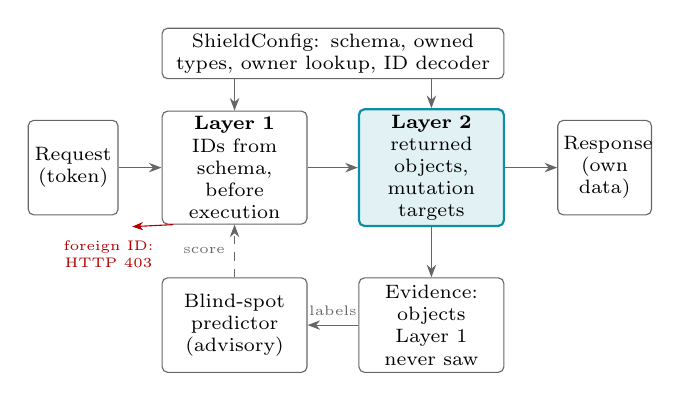
\begin{tikzpicture}[
  box/.style={draw=black!60, rounded corners=2pt, align=center, font=\scriptsize, minimum height=12mm, inner sep=2pt},
  acc/.style={box, draw=shieldteal, fill=shieldteal!12, line width=0.8pt},
  arr/.style={-{Stealth[length=1.6mm]}, black!60}
]
\node[box, text width=1.0cm] (req) at (0,0) {Request\\(token)};
\node[box, text width=1.7cm] (l1) at (2.05,0) {\textbf{Layer 1}\\IDs from schema,\\before execution};
\node[acc, text width=1.7cm] (l2) at (4.55,0) {\textbf{Layer 2}\\returned objects,\\mutation targets};
\node[box, text width=1.05cm] (resp) at (6.75,0) {Response\\(own data)};
\node[box, text width=4.2cm, minimum height=6mm] (cfg) at (3.3,1.45) {ShieldConfig: schema, owned types, owner lookup, ID decoder};
\node[box, text width=1.7cm] (pred) at (2.05,-2.0) {Blind-spot\\predictor\\(advisory)};
\node[box, text width=1.7cm] (ev) at (4.55,-2.0) {Evidence:\\objects Layer 1\\never saw};
\draw[arr] (req) -- (l1);
\draw[arr] (l1) -- (l2);
\draw[arr] (l2) -- (resp);
\draw[arr] (cfg.south -| l1) -- (l1);
\draw[arr] (cfg.south -| l2) -- (l2);
\draw[arr] (l2) -- (ev);
\draw[arr] (ev) -- node[above, font=\tiny]{labels} (pred);
\draw[arr, dashed] (pred) -- node[left, font=\tiny]{score} (l1);
\node[font=\tiny, text=red!70!black, align=center] at (0.45,-1.1) {foreign ID:\\HTTP 403};
\draw[-{Stealth[length=1.4mm]}, red!70!black] (l1.south west) ++(0.15,0) -- (0.75,-0.75);
\end{tikzpicture}
\caption{GraphQL-Shield. Layer 1 rejects requests naming foreign objects (HTTP 403); Layer 2 filters returned objects and blocks foreign writes, and records every object Layer 1 never evaluated, which trains the advisory predictor.}
\label{fig:arch}
\end{figure}

\subsection{Per-application configuration}
A \code{ShieldConfig} describes the protected application: its schema; which object types are owned, each mapped to an ownership key; an owner-lookup function from (key, identifier) to owner; the argument names that carry identifiers and a decoder for them (for example, Relay global identifiers); and targets for mutations whose return type does not reveal what they change. Everything else is derived from the schema. For our demo application this is two owned types and one mutation entry the schema cannot supply (\code{deleteResource} returns \code{Boolean}).

\subsection{Layer 1: schema-aware pre-execution gate}
Layer 1 parses the request before the engine runs and walks it against the schema. For every field with an identifier argument it takes the object type from the schema---the owned type the field returns or, for a root mutation, its configured target---rather than from the field's name. It resolves values as the engine will: literals, variables, declared defaults, lists, named and inline fragments, aliases, and each operation of a batch. A global identifier whose embedded type differs from the type the field expects is checked as both types, which defeats type confusion. One denial rejects the whole request with HTTP 403, so a write never starts.

\subsection{Layer 2: execution-time guard}
Layer 2 runs inside the engine as graphql-core middleware. Before a root mutation's resolver runs, it checks the target argument the engine actually coerced; a denial raises an error and the resolver never executes. After each resolver returns, it decides whether the value is an owned object from the field's GraphQL return type, not from the value's class, so it works with typed objects, dictionaries or ORM rows. A denied single object becomes \code{null}; a denied list item is removed before GraphQL enforces non-null types, so the caller keeps their own items. A mutation with no derivable or configured target is denied unless explicitly listed as unguarded.

\subsection{Cross-layer evidence}
Layer 1 marks every (type, identifier) it evaluated. Layer 2 writes an audit record only for objects Layer 1 never marked, so each such record is direct evidence of a Layer 1 coverage gap, and no decision is counted twice. When Layer 2 also denies such an object it records a blind-spot event: an attack only Layer 2 stopped.

\subsection{Self-supervised blind-spot predictor}
The coverage-gap records label requests without human effort. For each request Layer 1 allows, the predictor computes 17 structural features available before execution: depth, field count, relationship fields and chain depth, identifier arguments and how many Layer 1 resolved, nested lookups, variables and defaults, fragments, aliases, directives, batch size, mutation flag and caller role. It never sees ownership data or enforcement outcomes. An XGBoost classifier~\cite{xgboost} (120 trees, depth 4) predicts whether a request will reach objects Layer 1 cannot see, and SHAP contributions~\cite{shap} explain each prediction. At runtime the score is advisory: it is recorded and attached to later blind-spot events so predictions can be checked against live traffic, and it never changes a decision.

% ===================================================================
\section{Implementation}

GraphQL-Shield is implemented in Python on FastAPI and graphql-core~3.3, with SQLite (write-ahead logging) for ownership data and audit records. Layer~1 is a dependency on the protected route; Layer~2 is a Strawberry schema extension or, for any graphql-core server, \code{OwnershipMiddleware(config)}. Every request is limited to depth 10, 15 aliases, 2,000 tokens and 5 batched operations. Profiling showed that opening and closing database connections took about 75\% of a protected request's time (19 connections per relationship query), so connections are pooled and rolled back on return. The test suite has 317 tests.

We evaluate on two applications. The \emph{demo} application (Strawberry, code-first) has users, documents and folders with integer identifiers. The \emph{clinic} application shares no code with it: a schema-first SDL on plain graphql-core, dictionary resolvers, Relay global identifiers, and patients, records and prescriptions with independent owners, so a colleague's record can sit on another doctor's patient. In both, resolvers contain no authorization checks, and each exposes an unprotected endpoint used only as a baseline.

% ===================================================================
\section{Evaluation}

We address four questions. \textbf{RQ1:} does each layer stop BOLA alone, and do both together? \textbf{RQ2:} can cross-layer labels expose real Layer~1 gaps? \textbf{RQ3:} how does the approach compare with per-field rules, including under configuration mistakes? \textbf{RQ4:} what does enforcement cost? All experiments run in-process on temporary seeded databases on a Windows laptop with Python~3.13. The ablation, the tool comparison and the security tests are deterministic, so we report counts; latency and the predictor are repeated.

\subsection{RQ1: Layer ablation}\label{sec:ablation}
Table~\ref{tab:ablation} runs six attacks by one user against another user's objects under each layer combination. Layer~1 alone leaks relationship traversal, because no identifier of the child appears in the query; Layer~2 alone stops every attack but catches writes only at execution time. On a larger benchmark of 5,000 requests, the protected endpoint blocked all 2,267 BOLA requests and none of the legitimate ones. The clinic application, protected through its configuration alone (three owned types, two mutation entries), passes all 14 of its security tests, including type-confused global identifiers, one- and two-level relationship filtering, create and update mutations on another doctor's patient, and Layer~2 acting alone.

\begin{table}[t]
\caption{Layer ablation: the layer that stopped each attack}
\label{tab:ablation}
\centering
\footnotesize
\begin{tabular}{@{}lcccc@{}}
\toprule
Attack & Both & L1 only & L2 only & Neither \\
\midrule
Direct & L1 & L1 & L2 & leaked \\
Nested lookup & L1 & L1 & L2 & leaked \\
Inline fragment & L1 & L1 & L2 & leaked \\
Relationship & L2 & \textbf{leaked} & L2 & leaked \\
Batch & L1 & L1 & L2 & leaked \\
Update mutation & L1 & L1 & L2 & leaked \\
\bottomrule
\end{tabular}
\end{table}

\subsection{RQ2: Blind-spot discovery}
We generated 4,000 varied requests from four callers---literals, variables, variable defaults, aliases, directives, named and inline fragments, relationships, batches and mutations---ran each through the gateway, and labelled them from Layer~2's evidence. We compare the model with the hand-written rule for Layer~1's documented blind spot, ``flag queries containing a relationship field'' (Table~\ref{tab:discovery}).

\begin{table}[t]
\caption{Blind-spot discovery on 4,000 requests (random test split)}
\label{tab:discovery}
\centering
\footnotesize
\begin{tabular}{@{}lcccc@{}}
\toprule
 & \multicolumn{2}{c}{Before fix} & \multicolumn{2}{c}{After fix} \\
\cmidrule(lr){2-3}\cmidrule(lr){4-5}
 & Model & Rule & Model & Rule \\
\midrule
F1 (coverage gaps) & 1.000 & 0.639 & 1.000 & 1.000 \\
Attack recall & 100\% & 23.4\% & 100\% & 100\% \\
\midrule
Blocked by Layer 1 & \multicolumn{2}{c}{1,415} & \multicolumn{2}{c}{1,678} \\
Attacks only Layer 2 stopped & \multicolumn{2}{c}{401} & \multicolumn{2}{c}{138} \\
\bottomrule
\end{tabular}
\end{table}

The discovery run exposed a gap the rule did not encode: Layer~1 ignored variables' declared default values, so \code{query(\$id: Int = 102)} sent without variables reached object 102 unchecked. All 585 such requests (queries and mutations) were coverage gaps, and 263 were attacks stopped only by Layer~2. After we fixed Layer~1, attacks reaching only Layer~2 fell by 66\%, and the remaining gaps were relationship traversal, which the rule then matched. On a query family held out from training (relationships inside fragments) both reach F1~1.000. Over five further seeds of 2,000 requests on the fixed Layer~1, the model reached F1 $0.998\pm0.004$ and attack recall $1.000\pm0.000$, identical to the rule; $28.9\%\pm1.5\%$ of allowed requests had a coverage gap, $75.6\pm8.8$ attacks per seed were stopped only by Layer~2, and relationship-field count was the top feature in every seed. Scoring a request takes about 1.2\,ms.

\subsection{RQ3: Comparison with graphql-shield}\label{sec:comparison}
We rebuilt the demo schema, seed data and unchecked resolvers in Node.js and protected them with graphql-shield~7.6.5 in its documented style: argument rules on lookups, type-wide rules on owned types, and rules on each mutation. Both systems ran the same 13 attack and 5 benign scenarios, judged by one oracle: an attack leaks if a non-owned object is returned or the victim object changes; a benign request fails if the caller's own objects are missing.

\begin{table}[t]
\caption{Comparison with graphql-shield}
\label{tab:comparison}
\centering
\footnotesize
\begin{tabular}{@{}L{2.5cm}L{2.55cm}L{2.55cm}@{}}
\toprule
 & GraphQL-Shield & graphql-shield \\
\midrule
Attacks leaked & 0 / 13 & 0 / 13 \\
Legitimate requests failed & 0 / 5 & 1 / 5 \\
Configuration written & 2 owned types, 1 non-derivable mutation entry & 8 permission entries, 4 rule functions \\
\midrule
\multicolumn{3}{@{}l}{\emph{One configuration entry removed}} \\
Missing mutation entry & 0 leaks (derived or denied) & write executes (allow fallback) \\
Missing type entry & type unprotected (9/13 or 1/13 leak) & 0--1 leak (overlapping rules) \\
With deny fallback & --- & 0 leaks; 1--4 of 5 legitimate requests blocked \\
\bottomrule
\end{tabular}
\end{table}

graphql-shield's failure is null propagation: in \code{children: [ResourceType!]!}, denying the one foreign child cannot null that item, so the error nulls the whole folder and its owner loses their own two documents. Layer~2 removes the item before nullability is enforced. Under configuration mistakes neither approach dominates (Table~\ref{tab:comparison}): GraphQL-Shield needs a quarter of the configuration and fails closed on mutations, but an omitted owned type is a single point of failure; graphql-shield's overlapping per-field rules tolerate one missing read rule but require far more configuration and lose availability under null propagation.

\subsection{RQ4: Latency}
We measured each configuration with 30 warm-up requests, then 5 repeats of 200, reporting the mean with a 95\% confidence interval across repeats ($t$-distribution, 4 degrees of freedom). Fig.~\ref{fig:latency} compares both-layer latency before and after connection pooling, measured back to back on the same machine: pooling reduced it 2.9 to 4.8 times. With pooling, overhead over the unprotected endpoint was +78\% for an owned lookup (19.6\,ms, CI [18.3, 21.0]), +81\% for a relationship query (38.4\,ms, CI [35.7, 41.2]) and +60\% for an update (29.4\,ms, CI [26.8, 32.0]). These are in-process measurements on a laptop with background load; network latency would dilute the relative overhead.

\begin{figure}[t]
\centering
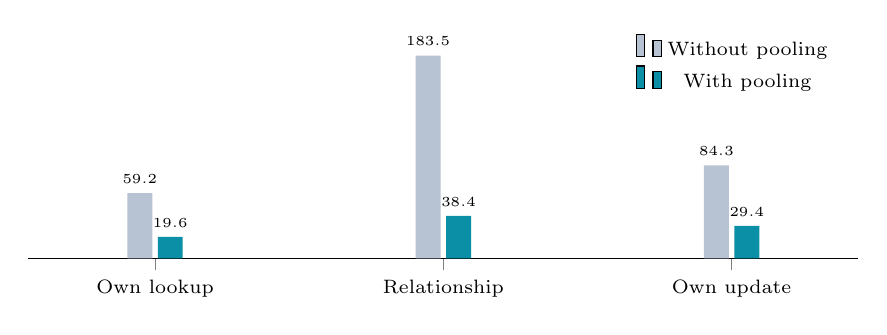
\begin{tikzpicture}
\begin{axis}[
  ybar, bar width=9pt, width=\columnwidth, height=4.6cm,
  ymin=0, ymax=215, ylabel={ms per request}, ylabel style={font=\scriptsize},
  symbolic x coords={Own lookup, Relationship, Own update}, xtick=data,
  tick label style={font=\scriptsize}, axis lines*=left, ytick=\empty, axis y line=none,
  nodes near coords, nodes near coords style={font=\tiny},
  legend style={font=\scriptsize, at={(0.98,0.97)}, anchor=north east, draw=none},
  enlarge x limits=0.22
]
\addplot[fill=shieldgrey, draw=none] coordinates {(Own lookup,59.2) (Relationship,183.5) (Own update,84.3)};
\addplot[fill=shieldteal, draw=none] coordinates {(Own lookup,19.6) (Relationship,38.4) (Own update,29.4)};
\legend{Without pooling, With pooling}
\end{axis}
\end{tikzpicture}
\caption{Mean both-layer latency per request, in-process, before and after connection pooling (5$\times$200 requests each).}
\label{fig:latency}
\end{figure}

% ===================================================================
\section{Discussion and Limitations}

\textbf{External validity.} Both applications and all attack scenarios were built by the authors. The results show the mechanism works on these applications, not that it generalises; evaluation on third-party applications and with independently written attacks is future work.

\textbf{Near-deterministic predictor.} In our applications a coverage gap follows almost entirely from query structure, so F1 near 1.0 reflects an easy target rather than real-world accuracy. Our claim concerns the method: cross-layer disagreement labels blind spots for free and the model names their causes. One discovery supports it; once fixed, the model adds no accuracy over the rule.

\textbf{Configuration as a single point of failure.} An owned type left out of the configuration is unprotected by both layers. A startup check that flags schema types with owner-like fields but no ownership entry would mitigate this.

\textbf{Policy, measurement and deployment.} Only owner-or-administrator access is supported; sharing, teams and attribute-based rules fit naturally into Layer~2's per-object check. Latency was measured in-process on a laptop. graphql-shield was reimplemented on a copy of our schema in its documented style; other rule sets could perform differently. Layer~1 runs in the application process rather than as a separate proxy.

% ===================================================================
\section{Conclusion}

Enforcing GraphQL object ownership at two independent points lets a gateway stop BOLA in every form we tested and measure its own blind spots. A pre-execution layer alone misses objects reached through relationships; an execution-time layer catches them and records each object the first layer never saw. Treated as free training labels, these records let a model find a real bypass of the first layer that a hand-written rule missed, and the fix cut attacks reaching only the execution-time layer by 66\%. The layers are configured from the schema and a small ownership map, protect a second unrelated application, avoid the availability loss that per-field rules suffer under null propagation, and cost 60--81\% latency in-process after connection pooling. Evaluating on third-party applications with independently written attacks is the next step.

\bibliographystyle{IEEEtran}
\bibliography{references}

\end{document}
